\documentclass[conference]{IEEEtran}
\IEEEoverridecommandlockouts
% The preceding line is only needed to identify funding in the first footnote. If that is unneeded, please comment it out.
\usepackage{cite}
\usepackage{amsmath,amssymb,amsfonts}
\usepackage{algorithmic}
\usepackage{graphicx}
\usepackage{textcomp}
\usepackage{xcolor}

\usepackage[utf8]{vietnam}

\usepackage{amsthm}

\usepackage{tabularray}
% \usepackage{ntheorem}
\newtheoremstyle{theoremst}% name of the style to be used
  {\topsep}% measure of space to leave above the theorem. E.g.: 3pt
  {\topsep}% measure of space to leave below the theorem. E.g.: 3pt
  {\normalfont}% name of font to use in the body of the theorem
  {0pt}% measure of space to indent
  {\bfseries}% name of head font
  {.}% punctuation between head and body
  { }% space after theorem head; " " = normal interword space
  {\thmname{#1}\thmnumber{ #2}\textnormal{\thmnote{ (#3)}}}

\newtheoremstyle{examplest}% name of the style to be used
  {\topsep}% measure of space to leave above the theorem. E.g.: 3pt
  {\topsep}% measure of space to leave below the theorem. E.g.: 3pt
  {\normalfont}% name of font to use in the body of the theorem
  {0pt}% measure of space to indent
  {\bfseries}% name of head font
  {\\}% punctuation between head and body
  { }% space after theorem head; " " = normal interword space
  {\thmname{#1}\thmnumber{ #2}\textnormal{\thmnote{ (#3)}}}
  
\theoremstyle{theoremst}
\newtheorem{definition}{Định nghĩa}[section]
\newtheorem{theorem}{Định lý}[section]


\def\BibTeX{{\rm B\kern-.05em{\sc i\kern-.025em b}\kern-.08em
    T\kern-.1667em\lower.7ex\hbox{E}\kern-.125emX}}
\begin{document}


\title{MAGNN: Metapath Aggregated Graph Neural Network for
Heterogeneous Graph Embedding\\
{\footnotesize \textsuperscript{}Giảng viên hướng dẫn: TS. Đỗ Thị Thanh Hà}
\thanks{Identify applicable funding agency here. If none, delete this.}
}

\author{\IEEEauthorblockN{ Nguyễn Mạnh Linh}
% \IEEEauthorblockA{\textit{dept. name of organization (of Aff.)} \\
% \textit{name of organization (of Aff.)}\\
% City, Country \\
% email address or ORCID}
\and
\IEEEauthorblockN{Nguyễn Đức Thịnh}
% \IEEEauthorblockA{\textit{dept. name of organization (of Aff.)} \\
% \textit{name of organization (of Aff.)}\\
% City, Country \\
% email address or ORCID}
% \and
% \IEEEauthorblockN{3\textsuperscript{rd} Given Name Surname}
% \IEEEauthorblockA{\textit{dept. name of organization (of Aff.)} \\
% \textit{name of organization (of Aff.)}\\
% City, Country \\
% email address or ORCID}
% \and
% \IEEEauthorblockN{4\textsuperscript{th} Given Name Surname}
% \IEEEauthorblockA{\textit{dept. name of organization (of Aff.)} \\
% \textit{name of organization (of Aff.)}\\
% City, Country \\
% email address or ORCID}
% \and
% \IEEEauthorblockN{5\textsuperscript{th} Given Name Surname}
% \IEEEauthorblockA{\textit{dept. name of organization (of Aff.)} \\
% \textit{name of organization (of Aff.)}\\
% City, Country \\
% email address or ORCID}
% \and
% \IEEEauthorblockN{6\textsuperscript{th} Given Name Surname}
% \IEEEauthorblockA{\textit{dept. name of organization (of Aff.)} \\
% \textit{name of organization (of Aff.)}\\
% City, Country \\
% email address or ORCID}
}

\maketitle

\begin{abstract}
Một lượng lớn các đồ thị hay mạng trong thực tế vốn dĩ không đồng nhất, có nhiều loại nút và nhiều loại quan hệ. Embedding đồ thị không đồng nhất là việc embed từ cấu trúc lớn và nhiều thông tin của đồ thị về biểu diễn nút trong không gian thấp chiều. Các mô hình đã tồn tại tường định nghĩa metapaths trong một đồ thị không đầu nhất để ghi lại các quan hệ và định hướng lựa chọn "hàng xóm". Tuy nhiên các mô hình này bỏ qua đặc trưng của từng nút mà tìm hiểu ngay lập tức các nút trên metapath hoặc chỉ xem xét một metapath. Để khắc phục ba giới hạn này, tác giả đề xuất một mô hình mới là \textit{Metapath Aggregated
Graph Neural Network} (MAGNN) để tăng tốc hiệu năng cuối cùng. Đặc biệt, MAGNN sử dụng ba thành phần chính, biến đổi nội dung của nút thành các thuộc tính đóng gói của nút đầu vào, tổng hợp intra-metapath để kết hợp các nút ngữ nghĩa trung gian và tổng hợp inter-metapath để kết hợp thông tin từ nhiều metapaths. Các thí nghiệm được thực hiện trên ba bộ dữ liệu đồ thị không đồng nhất trong thực tế để phân loại nút, phân cụm nút và dự đoán liên kết chỉ ra rằng MAGNN đạt được kết quả dự đoán chính xác hơn so với các mô hình state-of-the-art hiện tại .
\end{abstract}

% \begin{IEEEkeywords}
% component, formatting, style, styling, insert
% \end{IEEEkeywords}

\section{Giới thiệu}
Nhiều bộ dữ liệu thực tế được biểu diễn với cấu trúc dữ liệu đồ thị, trong đó các đối tượng và quan hệ giữa chúng được biểu diễn bằng các nút và cạnh. Các ví dụ bao gồm mạng xã hội [14, 29], hệ thống vật lý [2, 10], mạng giao thông [18, 34], mạng trích dẫn [1, 14, 16], hệ thống gợi ý [26, 35], đồ thị tri thức [3, 24], ... Bản chất non-Euclidean của đồ thị khiến chúng khó được mô hình hóa bằng các mô hình học máy truyền thống. Với tập lân cận của mỗi nút, không hề có thứ tự hoặc giới hạn về kích thước, Tuy nhiên, hầu hết các mô hình thống kê giả định rằng một đầu vào có thứ tự và kích thước cố định trong không gian Euclid. Do đó, sẽ thuận tiện nếu các nút có thể được biểu diễn bằng các vector thấp chiều trong không gian Euclid và từ đó có thể lấy làm đầu vào của mô hình học máy khác. 

Các kĩ thuật embed đồ thị khác nhau được đề xuất cho cấu trúc dữ liệu đồ thị. LINE [25] sinh node embedding dựa vào các nút gần nhất và gần thứ 2. Các phương pháp dựa trên bước ngẫu nhiên (Random-walk) bao gồm DeepWalk [21], node2vec [13] và TADW [32] sinh dãy nút được sinh ra bởi các bước ngẫu nhiên đến một mô hình skip-gram [19] để học node embeddings. Với sự phát triển nhanh chóng của deep learning, mạng neuron đồ thị (Graph neural networks - GNNs) được đề xuất, mô hình học các biểu diễn đồ thị bằng việc sử dụng các lớp neuron được thiết kế đặc biệt. Spectral-based GNNs bao gồm ChebNet [8] và GCN [16] biểu diễn các toán tử tích chập đồ thị trong miền Fourier của một đồ thị đầy đủ. Các mô hình dựa trên spatial, bao gồm GraphSAGE [14], GAT [28] và nhiều biến thể khác [17, 34, 45], giải quyết các vấn đề xung quanh khả năng mở rộng và khả năng tổng quát hóa của các mô hình dựa trên phổ bằng cách biểu diễn các phép toán tích chập đồ thị trực tiếp trên miền đồ thị. 

Mặc dù GNNs đã đạt được những kết quả tốt nhất trong nhiều bài toán, hầu hết các mô hình dựa trên GNN giả định rằng đầu vào là đồ thị đồng nhất với chỉ một loại nút và một loại cạnh. Hầu hết đồ thị trong thực tế bao gồm nhiều loại nút và cạnh tương ứng với các thuộc tính trong các không gian thuộc tính khác nhau. Ví dụ, một mạng đồng tác giả chứa ít nhất hai loại nút, cụ thể là các tác giả và bài báo. Các thuộc tính của tác giả có thể bao gồm nơi làm việc, trích dẫn và lĩnh vực nghiên cứu. Thuộc tính của bài báo bao gồm từ khóa, địa điểm, năm phát hành ... Tác giả gọi loại đồ thị này là \textit{mạng thông tin không đồng nhất} (HINs) hoặc \textit{đồ thị không đồng nhất.}
 Sự không đồng nhất trong cả cấu trúc biểu diễn và nội dung của nút khiến GNN gặp khó khăn trong việc mã hóa thông tin vào không gian vector thấp chiều. 

 Hầu hết các phương pháp nhúng đồ thị không đồng nhất hiện có dựa trên ý tưởng về metapaths. Một \textit{metapath} là một trình tự có thứ tự của các loại nút và loại cạnh được xác định trên lược đồ mạng, mô tả mối quan hệ tổng hợp giữa các loại nút liên quan. Ví dụ một mạng với tác giả, bài báo và dịa điểm, \textit{Tác giả-Bài báo-Tác giả} (APA) và \textit{Tác giả-Bài báo-Địa điểm-Bài báo-Tác giả} (APVPA) là các metapaths mô tả mối quan hệ khác nhau giữa các tác giả. Metapath APA tương ứng với hai đồng tác giả, trong khi APVPA tương ứng với hai tác giả xuất bản bài báo cùng địa điểm. Do đó, ta có thể xem metapath là khoảng cách gần bậc cao giữa 2 nút. Do GNNs truyền thống xử lý tất cả các nút như nhau, chúng không thể mô hình hóa cấu trúc phức tạp và thông tin có nghĩa trong đồ thị không đồng nhất.


 Mặc dù các phương pháp nhúng dựa trên metapath này hoạt động tốt hơn phương pháp nhúng mạng truyền thống trên các bài toán khác nhau, chẳng hạn như phân loại nút và dự đoán liên kết, chúng vẫn có ít nhất một trong những hạn chế sau. (1) Mô hình không sử dụng đặc trưng về nội dung nút nên nó hiếm khi hoạt động tốt với các đồ thị không đồng nhất với nút có nội dung nhiều đặc trưng (ví dụ metapath2vec [9], ESim [22], HIN2vec [11], HERec [23]). (2) Mô hình loại bỏ tất cả các nút trên metapath, chỉ xem xét 2 nút cuối dẫn đến mất thông tin (ví dụ HERec [23] and HAN [31]). (3) Mô hình dựa trên một metapath duy nhất để nhúng đồ thị không đồng nhất. Do đó, mô hình yêu cầu một quá trình chọn metapath thủ công và mất đi các đặc điểm của thông tin từ các metapaths khác dẫn đến hiệu năng không tối ưu (ví dụ metapath2vec [9]). 

 Để giải quyết các hạn chế này, tác giả đề xuất một mạng neuron tổng hợp metapath (\textit{Metapath Aggregated Graph Neural Network - MAGNN}) mới cho việc nhúng đồ thị không đồng nhất. MAGNN giải quyết tất cả các vấn đề được mô tả ở trên bằng cách áp dụng chuyển đổi nội dung nút, tổng hợp nội intra-metapath và tổng hợp inter-metapath để tạo nút nhúng. Cụ thể, MAGNN trước tiên áp dụng biến đổi tuyến tính theo loại cụ thể để chiếu các thuộc tính nút không đồng nhất với số chiều có thể không bằng nhau cho các loại nút khác nhau, cho cùng một không gian latent. Tiếp theo, MAGNN áp dụng intra-metapath với cơ chế chú ý [28] cho mọi metapath. Trong tổng hợp intra-metapath này, mỗi nút đích trích xuất và kết hợp thông tin từ các cấu hình metapath kết nối với nút lân cận dựa trên metapath của nó. Bằng cách này, MAGNN nắm bắt được thông tin về cấu trúc và ngữ nghĩa của các đồ thị không đồng nhất từ cả các nút lân cận và bối cảnh metapath giữa chúng. Sau khi tổng hợp intra-metapath, MAGNN tiếp tục tiến hành tổng hợp inter-metapath bằng cách sử dụng cơ chế chú ý để hợp nhất các latent vector thu được từ nhiều metapaths vào các nút nhúng cuối cùng. Bằng cách tích hợp nhiều metapaths, mô hình của tác giả có thể học ngữ nghĩa toàn diện ẩn giấu trong đồ thị không đồng nhất. 

Tóm lại, bài báo này có một số đóng góp chính:
\begin{itemize}
  \item[] (1) Tác giả đề xuất một mạng neuron đồ thị mới  dựa trên tổng hợp metapath để nhúng nhúng đồ thị không đồng nhất.
  \item[] (2) Thiết kế một số hàm mã hóa tiềm năng để trích xuất thông tin từ các cấu hình metapaths, bao gồm trường hợp dựa trên ý tưởng phép xoay quan hệ trong không gian phức [24].
  \item[] (3) Tác giả tiến hành nhiều thí nghiệm trên các tập dữ liệu IMDb và DBLP để phân loại và phân cụm nút cũng như dùng tập Last.fm để đánh giá dự đoán liên kết và hiệu suất của mô hình. Thí nghiệm trên tất cả các tập dữ liệu này và các bài toán chỉ ra rằng nhúng nút được học bởi MAGNN luôn tốt hơn các mô hình tiên tiến nhất hiện tại (SOTA).
\end{itemize}


\section{Sơ lược}
Trong phần này, tác giả đưa ra các định nghĩa chuẩn của một số thuật ngữ quan trọng liên quan đến đồ thị không thuần nhất. Minh họa trong hình 1. Bên cạnh đó bảng 1 tóm tắt các kí hiệu được sử dụng nhiều trong báo cáo để thuận tiện cho việc tra cứu nhanh.

\begin{definition}
\textbf{Đồ thị không đồng nhất.} Một đồ thị không đồng nhất được định nghĩa là một đồ thị $\pmb{\mathcal{G}} = (\pmb{\mathcal{V}}, \pmb{\mathcal{E}})$ với ánh của loại nút $\phi: \pmb{\mathcal{V}} \to \pmb{\mathcal{A}}$ và ánh xạ của loại cạnh $\psi: \pmb{\mathcal{E}} \to \pmb{\mathcal{R}}$. $\pmb{\mathcal{A}}$ và $\pmb{\mathcal{R}}$ lần lượt là các tập loại nút và loại cạnh với $|\pmb{\mathcal{A}}| + |\pmb{\mathcal{R}}| > 2$.
\end{definition}

\begin{definition}
  \textbf{Metapath.} Một metapath $P$ được định nghĩa là một đường đi lập thành từ $A_1  \xrightarrow{R_1} A_2  \xrightarrow{R_2} ... \xrightarrow{R_l} A_{l+1}$ (viết tắt là $A_1 A_2 ... A_{l+1}$) mô tả một quan hệ tổng hợp $R = R_1 \circ R_2 \circ ... \circ R_l$ giữa các loại nút $A_1$ và $A_{l+1}$, trong đó $\circ$ là toán tử tổng hợp trên các quan hệ.
\end{definition}

\begin{definition}
  \textbf{Cấu hình metapath.} Cho một metapath $P$ của một đồ thị không đồng nhất, một cấu hình metapath $p$ của $P$ được định nghĩa là một dãy các nút trong đồ thị theo lược đồ được xác định bởi $P$.
\end{definition}

\begin{definition}
  \textbf{Lân cận dựa trên metaptah.} Cho một metapath $P$ của một đồ thị không đồng nhất, các lân cận dựa trên metapath $\pmb{\mathcal{N}}_\upsilon ^ P$ của một nút $\upsilon$ được định nghĩa là tập hợp các nút liên kết với nút $\upsilon$ qua các cấu hình metapath của $P$. Một lân cận được kết nối bởi hai cấu hình metapath khác nhau được đánh giá như hai nút khác nhau trong $\pmb{\mathcal{N}}_\upsilon ^ P$. Lưu ý rằng $\pmb{\mathcal{N}}_\upsilon ^ P$ bao gồm chính nút $\upsilon$ nếu $P$ đối xứng.

  Ví dụ, xem xét tập dữ liệu UATA trong hình 1, nghệ sĩ \textit{Queen} là một lân cân dựa trên metapath của người dùng \textit{Bob}. Hai nút này được kết nối thông qua cấu hình metapath \textit{Bob-Beatles-Rock-Queen}. Hơn nữa, chúng ta có thể tham chiếu tới \textit{Beatles} và \textit{Rock} như là các nút trung gian trên cấu hình metapath này.
\end{definition}

\begin{definition}
  \textbf{Đồ thị dựa trên metapath.} Cho một metapath $P$ của một đồ thị không đồng nhất $\pmb{\mathcal{G}}$, đồ thị dựa trên metapath $\pmb{\mathcal{G}}^P$ là một đồ thị được xây dựng bởi tất cả các cặp lân cận dựa trên metapath $P$ trong đồ thị $\pmb{\mathcal{G}}$. Lưu ý rằng $\pmb{\mathcal{G}}^P$ là đồng nhất nếu $P$ đối xứng.
\end{definition}

\begin{definition}
  \textbf{Biểu diễn đồ thị không đồng nhất.} Cho một đồ thị không đồng nhất $\pmb{\mathcal{G}} = (\pmb{\mathcal{V}}, \pmb{\mathcal{E}})$ với các ma trận thuộc tính nút $\pmb{X}_{A_i} \in \mathbb{R} ^ {|\pmb{\mathcal{V}}_{A_i}| \times d_{A_i}}$ của các loại nút $A_i \in \pmb{\mathcal{A}}$, biểu diễn đồ thị không đồng nhất là việc học các biểu diễn nút $d$ chiều $\pmb{h}_{\upsilon} \in \mathbb{R}^d$ với mọi $\upsilon \in \pmb{\mathcal{V}}$ với $d \ll |\pmb{\mathcal{V}}|$ có thể ghi lại thông tin cấu trúc và ngữ nghĩa liên quan đến $\pmb{\mathcal{G}}$.
\end{definition}

\begin{figure*}
  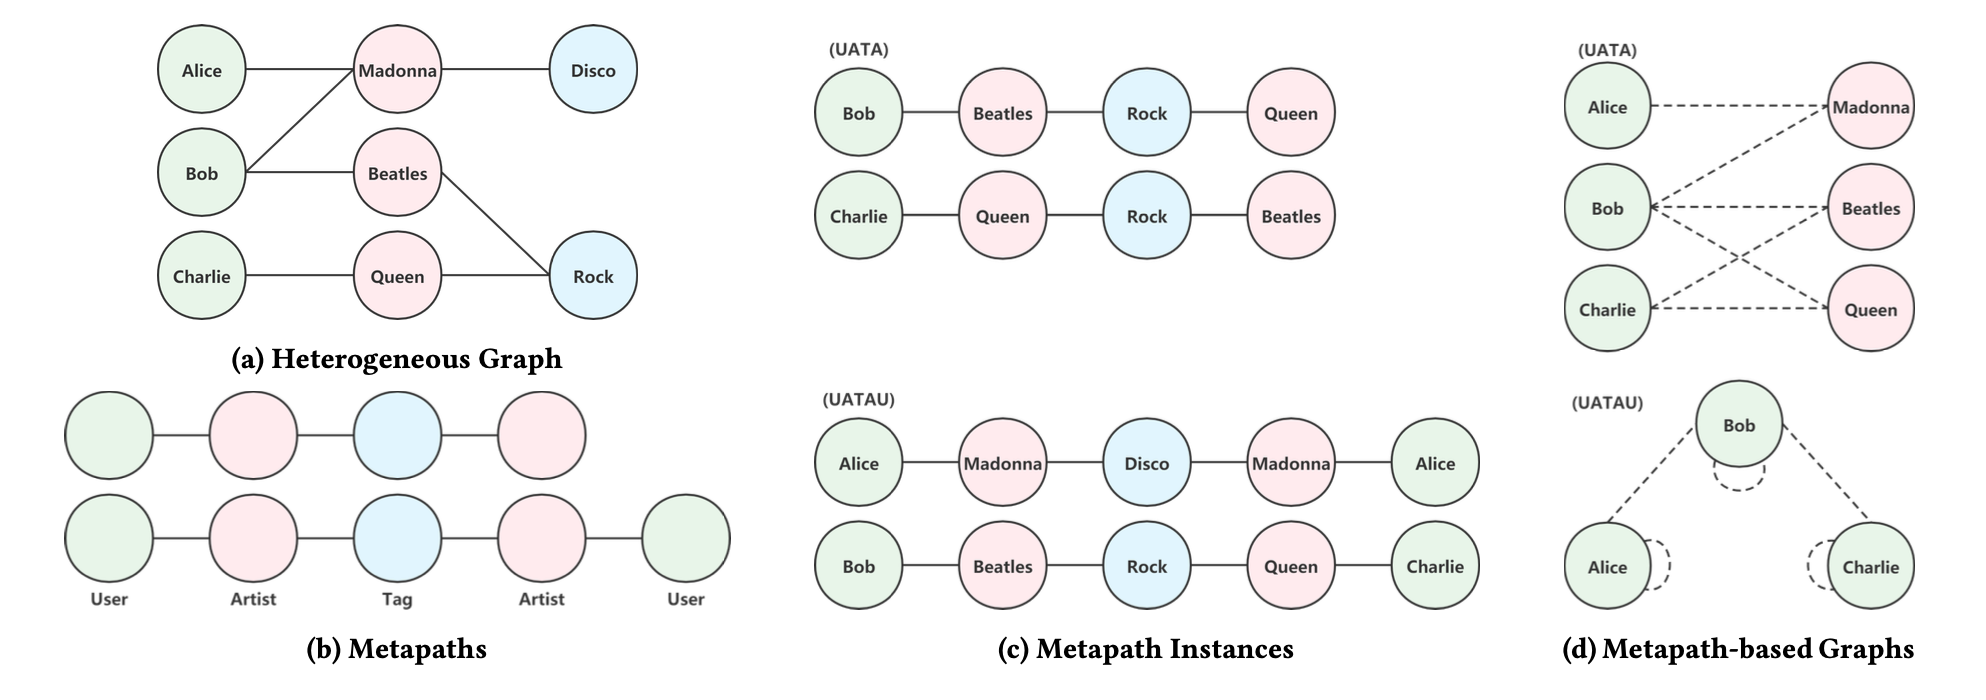
\includegraphics[width=\textwidth]{figs/fig1.png}
  \caption{Minh họa các thuật ngữ được định nghĩa trong Phần 2. (a) Một ví dụ về đồ thị không đồng nhất với ba loại nút (người dùng, nghệ sĩ, thẻ). (b) metapath Người dùng-Nghệ sĩ-Thẻ-Nghệ sĩ (UATA) và metapath Người dùng-Nghệ sĩ-Thẻ-Nghệ sĩ-Người dùng (UATAU). (c) Ví dụ các cấu hình metapath của UATA, UATAU. (d) Đồ thị dựa trên metapath cho UATA và UATAU.}
\end{figure*}





\section{Nghiên cứu liên quan}
Trong phần này, tác giả xem lại các nghiên cứu về học biểu diễn đồ thị liên quan tới mô hình của tác giả. Chúng được chia thành hai phần nhỏ: phần đầu tóm tắt các nỗ lực nghiên cứu về GNN cho việc nhúng đồ thị, phần sau giới thiệu các phương pháp nhúng đồ thị cho các đồ thị không đông nhất.

\subsection{Mạng neuron đồ thị}
Mục tiêu của một GNN là học một biểu diễn vector thấp chiều $\pmb{h}_{\upsilon}$ cho mọi nút $\upsilon$, cách được sử dụng cho nhiều tác vụ downstream, ví dụ như phân loại nút, phân cụm nút và dự đoán liên kết. Lý do đằng sau điều này là mỗi nút được xác định một cách tự nhiên bởi các đặc trưng và khu vực lân cận của nó. Theo ý tưởng này và dựa trên quá trình xử lý tín hiệu đồ thị, GNNs dựa trên phổ được phát triển để thực hiện tích chập đồ thị trong miền Fourier của một đồ thị. ChebNet [8] sử dụng các đa thức Chebusev để lọc các tín hiệu đồ thị (đặc trưng nút) trong miền Fourier của đồ thị. Một mô hình có ảnh hưởng khác thuộc loại này là GCN [16], nó ràng buộc và đơn giản hóa các tham số của ChebNet để giảm bớt vấn đề overfitting và cải thiện hiệu năng. Tuy nhiên, GNNs dựa trên phổ có khả năng mở rộng và tổng quát kém vì chúng yêu cầu toàn bộ đồ thị làm đầu vào cho mọi lớp và các bộ lọc đã được học của chúng phụ thuộc vào cơ sở riêng của Laplacian của đồ thị, liên quan chặt chẽ đến cấu trúc đồ thị cụ thể.

GNNs dựa trên spatial đã được đề xuất để khắc phục những giới hạn này. GNNs kiểu này định nghĩa các tích chập một cách trực tiếp trong miền đồ thị bằng cách tổng hợp thông tin từ các lân cận của mỗi nút, giống như các toán tử tích chập trong mạng tích chập xử lý dữ liệu hình ảnh. GraphSAGE [14], một framework GNN dựa trên spatial được tạo ra dựa trên khái niệm chung về các hàm tổng hợp để tạo các nút nhúng hiệu quả. Các mẫu hàm tổng hợp và biến đổi một lân cận của nút mục tiêu và do đó tạo điều kiện huấn luyện song song và tổng quát hóa cho các nút hoặc đồ thị ẩn. Rất nhiều biến thể của GNN dựa trên spatial được đề xuất dựa trên ý tưởng này. Lấy cảm ứng từ Transformer [27], GAT [28] kết hợp cơ chế chú ý vào hàm tổng hợp để đưa vào độ quan trọng tương đối của thông tin của mỗ lân cận từ góc nhìn của nút đích. GGNN [17] thêm một thành phần lặp có kiểm soát (GRU) [7] vào hàm tổng hợp bằng cách xử lý thông tin vùng lân cận được tổng hợp làm đầu vào cho GRU của bước thời gian hiện tại. GaAN [34] kết hợp GRU với cơ chế chú ý nhiều đầu để  thỏa mãn không thời gian đồ thị. STAR-GCN [35] dử dụng nhiều bộ mã hóa-giải mã GCN để
tăng hiệu suất dự đoán xếp hạng. 

Tất cả các GNN được đề cập ở trên đều được xây dựng cho các đồ thị đồng nhất hoặc được thiết kế cho một số đồ thị với cấu trúc đặc biệt như là trong các hệ thống gợi ý người dùng - sản phẩm. Do hầu hết các GNNs hiện tại hoạt động trên đặc trưng của các nút trong cùng không gian nhúng được chia sẻ, chúng không thể đáp ứng một cách tự nhiên với các đồ thị không đồng nhất với các đặc trung nút nằm trên các không gian khác nhau.

\subsection[short]{Nhúng đồ thị không đồng nhất}
Nhúng đồ thị không đồng nhất nhằm mục đích chiếu các nút từ một đồ thị không đồng nhất vào một không gian vector thấp chiều. Chủ đề thách thức này thu hút rất nhiều nghiên cứu. Ví dụ, metapath2vec [9] sinh các bước ngẫu nhiên được hướng dẫn bởi một meta-path đơn, thứ sau đó được lấy làm đầu vào cho mô hình skip-gram [19] để sinh các nút nhúng. Với metapaths được định nghĩa trước, ESim [22] sinh các nút nhúng bằng cách học từ các cấu hình metapath mẫu âm và dương. HIN2vec [11] thực hiện nhiều tác vụ huấn luyện để học các biểu diễn của nút và metapaths của một đồ thị không đồng nhất. Cho một metapath, HERec [23] chuyển đổi một đồ thị không đồng nhất thành một đồ thị đồng nhất dựa trên các lân cận metapath-based và áp dụng mô hình DeepWalk  để học nhúng nút của các loại mục tiêu. Giống như HERec, HAN [31] chuyển đổi một đồ thị không đồng nhất thành nhiều đồ thị đồng nhất dựa trên metapath theo cách tương tự nhưng sử dụng một kiến trúc mạng chú ý đồ thị để tổng hợp thông tin từ các lân cận và thúc đẩy cơ chế chú ý để kết hợp nhiều metapaths. Một mô hình khá là PME [6] học nhúng nút bằng các chiếu chúng vào các không gian quan hệ tương ứng và tối ưu hóa tiệm cận giữa các nút được chiếu.

Tuy nhiên, tất cả các phương pháp nhúng đồ thị không đồng nhất được giới thiệu ở trên có những hạn chế là bỏ qua các đặc trưng về nội dung của nút, loại bỏ tất cả các nút trung gian dọc theo metapath hoặc chỉ sử dụng một metapath duy nhất. Mặc dù chúng có thể được cải thiện dựa trên hiệu năng của các phương pháp nhúng đồ thị không đồng nhất cho một số bộ dữ liệu đồ thị không đồng nhất, vẫn có thể làm tốt hơn bằng cách khai thác toàn diện hơn các thông tin trong đồ thị không đồng nhất. 

\section{Phương pháp}
Trong phần này, tác giả mô tả một mạng neuron đồ thị tổng hợp metapath mới (MAGNN) để nhúng đồ thị không đồng nhất. MAGNN được xây dựng bởi 3 thành phần chính: biến đổi nội dung nút, tổng hợp hợp intra-metapath và tổng hợp inter-metapath. Hình 2 minh họa việc tạo nhúng của một nút. Các quá trình lan truyền tiến được chỉ ra trong thuật toán 1.

\subsection{Biến đổi nội dung nút}
Với một đồ thị không đồng nhất liên kết với các thuộc tính nút, các loại nút khác nhau có thể có chiều của các vector đặc trưng không bằng nhau. Kể cả chúng có số chiều bằng nhau thì chúng cũng nằm trên các không gian đặc trưng khác nhau. Ví dụ các bag-of-words vectors $n_1$ chiều của đoạn văn bản và các vectors biểu đồ cường độ $n_2$ chiều của hình ảnh không thể  trực tiếp hoạt động cùng nhau kể cả $n_1 = n_2$. Các vectors đặc trưng với các chiều khác nhau là một khó khăn khi tác giả xử lý chúng trong một framework thống nhất. Do đó, tác giả cần chieus các loại khác nhau của đặc trưng nút vào cùng một không gian vector latent trước.

Vì vậy trước khi đưa các vectors nút vào MAGNN, tác giả áp dụng phép biến đổi tuyến tính cho từng loại nút bằng cách chiếu các vector đặc trưng vào cùng một không gian latent. Với một nút $\nu \in \pmb{\mathcal{V}}_A$ của loại $A \in \pmb{\mathcal{A}}$, ta có
\begin{equation}
  \mathbf{h'}_{\nu} = \mathbf{W}_A \cdot \mathbf{x}^A_{\nu}
\end{equation}
trong đó $\mathbf{x}_{\nu} \in \mathbb{R}^{d_A}$ là vector đặc trưng gốc và $\mathbf{h'}_{\nu} \in \mathbb{R}^{d'}$ là vector lantent hình chiếu  của nút $\nu$. $\mathbf{W}_A \in \mathbb{R}^{d' \times d_A}$ là ma trận trọng số của các nút loại $A$.

Biến đổi nội dung nút giải quyết tính không đồng nhất của một đồ thị bắt nguồn từ các đặc trưng nội dung nút. Sau khi áp dụng tác động này, tất cả các đặc trưng chiếu của nút đều có cùng chiều, tạo điều kiện thuận lợi cho quá trình tổng hợp của thành phần tiếp theo của mô hình. 

\begin{figure*}
  \label{fig:02}
  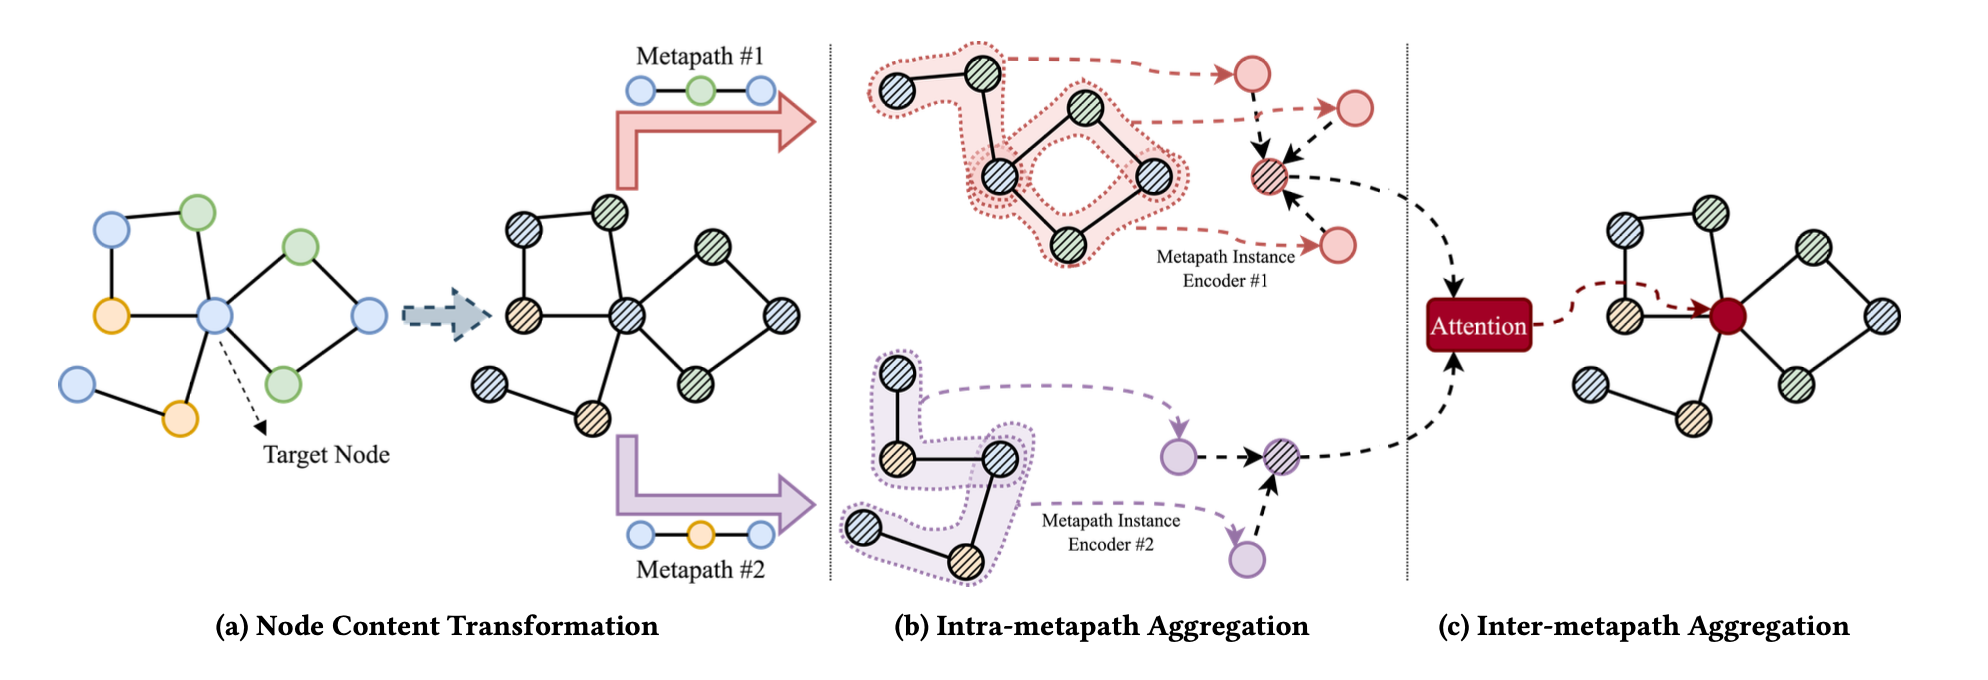
\includegraphics[width=\textwidth]{figs/fig2.png}
  \caption{Kiến trúc tổng thể của MAGNN}
\end{figure*}

\subsection{Tổng hợp intra-metapath}
Cho một metapath $P$, lớp tổng hợp intra-metapath học thông tin cấu trúc và ngữ nghĩa được nhúng trong nút mục tiêu, các lân cận dựa trên metapath và ngữ cảnh ở giữa bằng cách mã hóa cấu hình metapath của $P$. Gọi $P(\nu, u)$ là một cấu hình metapath kết nối nút mục tiêu $\nu$ và lân cận dựa trên metapath $u \in \pmb{\mathcal{N}}^P_{\nu}$, tác giả định nghĩa thêm  nút trung gian của $P(\nu, u)$ như sau $\{ m^{P(\nu, u)} \} = P(\nu, u) \backslash \{ \nu, u \}$. Tổng hợp intra-metapath sử dụng một bộ mã hóa cấu hình metapath để biến đổi tất cả các đặc trưng nút dọc theo một cấu hình metapath thành một vector duy nhất,
\begin{equation}
  \mathbf{h}_{P(\nu, u)} = f_{\theta} (P(\nu, u)) = f_{\theta} \left( \mathbf{h'}_{\nu}, \mathbf{h'}_{u}, \{ \mathbf{h'}_{t}, \forall t \in \{m^{P(\nu, u)}\} \} \right)
\end{equation}
trong đó, $\mathbf{h}_{P(\nu, u)} \in \mathbb{R}^{d'}$ có số chiều là $d'$. Để đơn giản, ta dùng $P(\nu, u)$ để biểu diễn một cấu hình đơn, mặc dù có thể có nhiều cấu hình kết nối 2 nút. Phần sau sẽ giới thiệu một vài lựa chọn của bộ mã hóa cấu hình metapath tốt.

Sau khi mã hóa các cấu hình metapath thành biểu diễn vector, tác giả áp dụng một lớp chú ý đồ thị [28] để  tính tổng trọng số các cấu hình metapath của $P$ liên quan đến nút đích $\nu$. Ý tưởng chính là các cấu hình metapath khác nhau sẽ đóng góp vào biểu diễn nút mục tiêu với mức độ khác nhau. Chúng ta có thể mô hình hóa điều này bằng cách học một trọng số chuẩn hóa quan trọng $\alpha^P_{\nu u}$ cho mỗi cấu hình metapath và sau đó tính tổng trọng số của tất cả các cấu hình:
\begin{equation}
  \begin{split}
    e^P_{\nu u} &= \text{LeakyReLU} (a^T_P \cdot [\mathbf{h'}_{\nu}\parallel \mathbf{h}_{P(\nu, u)}]), \\
  \alpha ^P_{\nu u} &= \frac{\text{exp}{e^P_{\nu u}}}{\sum _{s \in \pmb{\mathcal{N}}^P_{\nu}} \text{exp} (e^P_{\nu u})}, \\
  \mathbf{h}^P_{\nu} &= \sigma \left( \sum_{u \in \pmb{\mathcal{N}}^P_{\nu}} \alpha ^P_{\nu u} \cdot \mathbf{h}_{P(\nu, u)} \right).
  \end{split}
\end{equation}
Trong đó, $a_P \in \mathbb{R}^{2d'}$ là vector chú ý được tham số hóa cho metapath $P$ và $\parallel$ kí hiệu cho toán tử nối vector. $e^P_{\nu u}$ chỉ độ quan trọng của cấu hình metapath $P(\nu, u)$ đến nút $\nu$, nút sau đó được chuẩn hóa theo các lựa chọn $u \in \pmb{\mathcal{N}}^P_{\nu}$ sử dụng hàm softmax. Do trọng số chuẩn hóa $\alpha ^P_{\nu u}$ được lấy cho tất cả $u \in \pmb{\mathcal{N}}^P_{\nu}$, chúng được sử dụng để tính toán một tổ hợp có trọng số của các biểu diễn của các cấu hình metapath cho nút $\nu$. Cuối cùng, đầu ra chạy qua hàm kích hoạt $\sigma (\cdot)$.

Cơ chế chú ý cũng có thể được mở rộng thành nhiều nhánh, điều giúp ổn định quá trình học và giảm đi phương sai lớn từ tính không đồng nhất của đồ thị. Nghĩa là, chúng ta thực hiện $K$ cơ chế chú ý độc lập và sau đó nối đầu ra của chúng lại, kết quả thu được trong biểu thức sau:
\begin{equation}
  \mathbf{h}^P_{\nu} = \parallel ^K_{k=1} \sigma \left( \sum_{u \in \pmb{\mathcal{N}}^P_{\nu}} \left[ \alpha ^P_{\nu u} \right]_k \cdot \mathbf{h}_{P(\nu, u)} \right)
\end{equation} 
trong đó $\left[ \alpha ^P_{\nu u} \right]_k$ là trọng số chuẩn hóa của cấu hình metapath $P(\nu, u)$ đến nút $\nu$ tại nhánh chú ý thứ $k$.

Tóm lại, với các vector đặc trưng $\mathbf{h'}_{u} \in \mathbb{R}^{d'} \forall u \in \pmb{\mathcal{V}}$ và tập các metapaths $\pmb{\mathcal{P}}_A = {P_1, P_2, ..., P_M}$ bắt đầu hoặc kết thúc với loại nút $A \in \pmb{\mathcal{A}}$, tổng hợp của MAGNN sinh $M$ biểu diễn metapath-specific vector của nút đích $\nu \in \pmb{\mathcal{V}}_A$, kí hiệu là $\{ \mathbf{h}^{P_1}_{\nu}, \mathbf{h}^{P_2}_{\nu}, ... , \mathbf{h}^{P_M}_{\nu} \}$. Mỗi $\mathbf{h}^{P_1}_{\nu} \in \mathbb{R}^{d'}$ (giả sử $K=1$) có thể hiểu là tổng hợp của các cấu hình $P_i-\text{metapath}$ của nút $\nu$, thể hiện một khía cạnh của thông tin chứ chong nút $\nu$.

\subsection{Tổng hợp inter-metapath}
Sau khi tổng hợp dữ liệu nút và cạnh với mỗi metapath, chúng ta cần kết hợp thông tin của tất cả các metapath sử dụng một lớp tổng hợp inter-metapath. Bây giờ với một loại nút $A$, ta có $|\pmb{\mathcal{V}}_A|$ tập các latent vectors: $\{ \mathbf{h}^{P_1}_{\nu}, \mathbf{h}^{P_2}_{\nu}, ... , \mathbf{h}^{P_M}_{\nu} \}$ với $\nu \in \pmb{\mathcal{V}}_A$, với $M$ là số metapaths cho loại $A$. Một các tiếp cận tổng hợp inter-metapath trực tiếp là lấy trung bình element-wise của các vectors nút này. Ta mở rộng cách tiếp cận này bằng cách khai thác cơ chế chú ý để gán các trọng số khác nhau cho các metapaths khác nhau. Phép toán này là có lý vì các metapaths có đóng góp không giống nhau trong một đồ thị không đồng nhất.

Đầu tiên, ta cộng mỗi metapath $P_i \in \pmb{\mathcal{P}}_A$ bằng trung bình các vectors nút metapath-specific đã được biến đổi cho tất cả các nút $\nu \in \pmb{\mathcal{V}}_A$,
\begin{equation}
  \mathbf{s}_{P_i} = \frac{1}{|\pmb{\mathcal{V}}_A|} \sum_{\nu \in \pmb{\mathcal{V}}_A} \text{tanh} \left( \mathbf{M}_A \cdot \mathbf{h}^{P_i}_{\nu} + \mathbf{b}_A \right)
\end{equation}
trong đó, $\mathbf{M}_A \in \mathbb{R}^{d_m \times d'}$ và $\mathbf{b}_A \in \mathbb{R}^{d_m}$ là các tham số học.

Sau đó ta sử dụng cơ chế chú ý để  hợp nhất các vectors nút metapath-specific của $\nu$ như sau:
\begin{equation}
  \begin{split}
    e_{P_i} &= \mathbf{q}^T_A \cdot \mathbf{s}_{P_i}, \\
    \beta _{P_i} &= \frac{\text{exp}(e_{P_i})}{\sum_{P \in \pmb{\mathcal{P}}_A} \text{exp}(e_{P})}, \\
    \mathbf{h}^{\pmb{\mathcal{P}}_A}_{\nu} &= \sum_{P \in \pmb{\mathcal{P}}_A} \beta _{P} \cdot \mathbf{h}^P_{\nu}
  \end{split}
\end{equation}
trong đó, $\mathbf{q}_A \in \mathbb{R}^{d_m}$ laf vector chú ý tham số hóa cho loại nút $A$. $\beta _{P_i}$ có thể hiểu là độ đóng góp tương đối của metapath $P_i$ cho các nút loại $A$. Do $\beta _{P_i}$ được tính toán cho mỗi $P_i \in \pmb{\mathcal{P}}_A$, ta có thể tính tổng có trọng số tất cả các vectors nút metapath-specific của $\nu$.

Cuối cùng, MAGNN sử dụng một biến đổi tuyến tính bổ sung với một hàm phi tuyến để chiếu các nút nhúng vào không gian vector với số chiều đầu ra mong muốn:
\begin{equation}
  \mathbf{h}_{\nu} = \sigma \left( \mathbf{W}_0 \cdot \mathbf{h}^{\pmb{\mathcal{P}}_A}_{\nu} \right)
\end{equation}
trong đó, $\sigma (\cdot)$ là một hàm kích hoạt và $\mathbf{W}_0 \in \mathbb{R}^{d_0 \times d'}$ là một ma trận trọng số. Phép chiếu này là một tác vụ cụ thể. Nó có thể hiểu là một phân loại tuyến tính cho phân loại nút hoặc được coi là hình chiếu vào không gian với các độ đo sự tương tự của nút cho dự đoán liên kết. 

\subsection{Biểu diễn (mã hóa) cấu hình metapath}
Để mã hóa cấu hình metapath trong phần IV.B, ta xem xét ba hàm mã hóa khả dĩ sau: 

\begin{itemize}
  \item Mã hóa trung bình. Hàm này tính toán trung bình theo từng thành phần (element-wise) của nút dọc theo cấu hình metapath $P(v, u)$ :
\end{itemize}
\begin{equation}
  \mathbf{h}_{P(v, u)}=\operatorname{MEAN}\left(\left\{\mathbf{h}_{t}^{\prime}, \forall t \in P(v, u)\right\}\right).
\end{equation}

\begin{itemize}
  \item Mã hóa tuyến tính. Hàm này là một phiên bản mở rộng của mã hóa trung bình, trong đó việc mã hóa được thực hiện dựa trên các biến đổi tuyến tính:
\end{itemize}
\begin{equation}
    \mathbf{h}_{P(v, u)}=\mathbf{W}_{P} \cdot \operatorname{MEAN}\left(\left\{\mathbf{h}_{t}^{\prime}, \forall t \in P(v, u)\right\}\right).
\end{equation}

\begin{itemize}
  \item Mã hóa dựa trên phép quay có quan hệ. Ta xem xét mã hóa một cấu hình metapath dựa trên phép quay có quan hệ trong không gian phức, một phương pháp được đề xuất bởi RotatE [24] để biểu diễn đồ thị tri thức. Hàm mã hóa trung bình và tuyến tính được giới thiệu ở trên coi các cấu hình metapath như một tập hợp, và vì thế chúng bỏ qua thông tin được biểu diễn trong kiến trúc chuỗi của metapath. Trong khi đó, phép quay có quan hệ lại cho phép ta mô hình hóa kiểu tri thức đó. Biết $P(v, u)=\left(t_{0}, t_{1}, \ldots, t_{n}\right)$ with $t_{0}=u$ và $t_{n}=v$, let $R_{i}$ là mối quan hệ giữa nút  $t_{i-1}$ và nút $t_{i}$, gọi $\mathbf{r}_{i}$ là vector mối quan hệ của $R_{i}$, khi đó mã hóa dựa trên phép quay có quan hệ được thể hiện bởi công thức.
\end{itemize}
\begin{equation}
    \begin{aligned}
    & \mathbf{o}_{0}=\mathbf{h}_{t_{0}}^{\prime}=\mathbf{h}_{u}^{\prime}, \\
    & \mathbf{o}_{i}=\mathbf{h}_{t_{i}}^{\prime}+\mathbf{o}_{i-1} \odot \mathbf{r}_{i}, \\
    & \mathbf{h}_{P(v, u)}=\frac{\mathbf{o}_{n}}{n+1},
    \end{aligned}
\end{equation}
trong đó  $\mathbf{h}_{t_{i}}^{\prime}$ và $\mathbf{r}_{i}$ đều là các vector phức, $\odot$ là tích vô hướng. Ta có thể dễ giàng phân tích một vector thực có số chiều là $d^{\prime}$ thành một vector phức có số chiều là $d^{\prime} / 2$ bằng cách coi nửa đầu tiên của vector là phần thực và nửa sau là phần ảo.

\subsection{Huấn luyện mô hình}
Sau khi thực hiện các biến đổi thành phần đã giới thiệu ở các phần trước, ta sẽ thu được biểu diễn cuối cùng của các nút để phục vụ cho các bài toán khác tiếp theo. Tùy theo đặc điểm khác nhau của các bài toán và việc nhãn của các nút có sẵn hay không mà chúng ta có thể huấn luyện mô hình MAGNN theo 2 mô hình (paradigm) chính là học bán giám sát (semi-supervised learning) và học không giám sát (unsupervised learning).

Đối với trường hợp học bán giám sát, với thông tin có được từ một phần nhỏ các nút được gán nhãn, ta có thể học các tham số của mô hình để tối thiểu hóa hàm cross-entropy bằng phương pháp lan truyền ngược (backpropagation) hoặc gradient descent. Và từ đó học được cách biểu diễn nút cho đồ thị không đồng nhất sao cho bảo toàn được nhiều thông tin quan trọng nhất có thể. Hàm tổn thất cross-entropy cho trường hợp học bán giám sát được cho bởi công thức sau:
\begin{equation}
    \mathcal{L}=-\sum_{v \in \mathcal{V}_{L}} \sum_{c=1}^{C} \mathbf{y}_{v}[c] \cdot \log \mathbf{h}_{v}[c]
\end{equation}
trong đó $V_{L}$ là tập hợp các nút có nhãn, $C$ là số lượng phân lớp, $\mathbf{y}_{v}$ là vector one-hot thể hiện nhãn của nút $v$, và $\mathbf{h}_{v}$ là vector xác suất dự báo của nút $v$.

Đối với trường hợp học không giám sát thì ta không có bất kì nhãn của nút nào cả, khi đó ta có thể học các tham số của mô hình bằng cách tối thiểu hóa hàm tổn thất sau đây [20]:
\begin{equation}
    \mathcal{L}=-\sum_{(u, v) \in \Omega} \log \sigma\left(\mathbf{h}_{u}^{\top} \cdot \mathbf{h}_{v}\right)-\sum_{\left(u^{\prime}, v^{\prime}\right) \in \Omega^{-}} \log \sigma\left(-\mathbf{h}_{u^{\prime}}^{\top} \cdot \mathbf{h}_{v^{\prime}}\right),
\end{equation}
trong đó $\sigma(\cdot)$ là hàm sigmoid, $\Omega$ là tập hợp các cặp nút quan sát được (dương tính), $\Omega^{-}$ là tập hợp các cặp nút âm tính được lấy mẫu từ tất cả các cặp nút không quan sát được (phần bù của $\Omega$).

\begin{figure}
  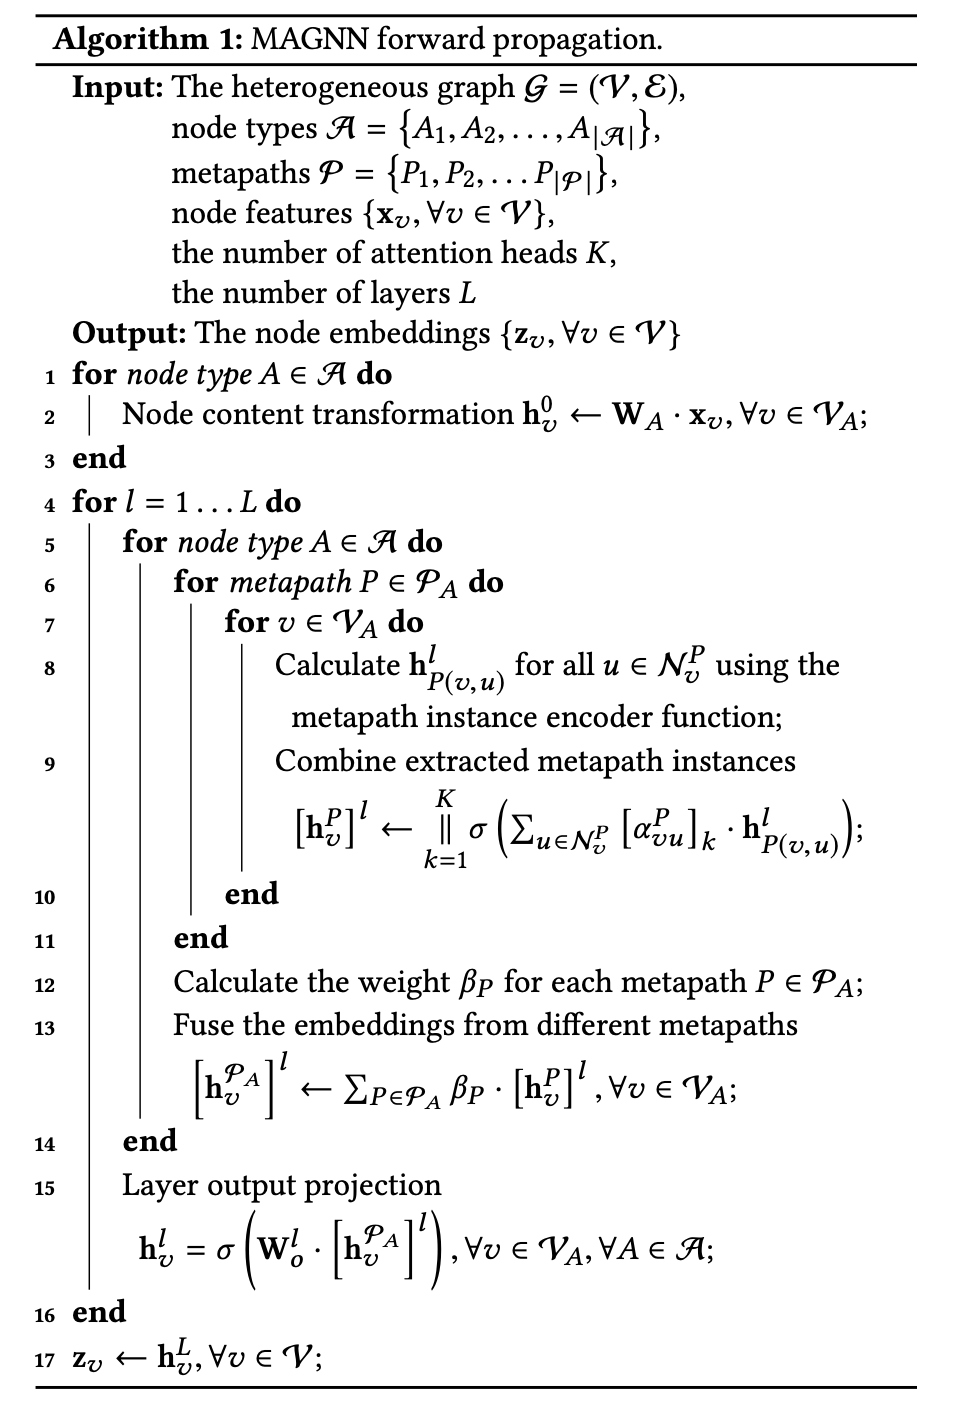
\includegraphics[width=\columnwidth]{figs/alg1.png}
\end{figure}


\section{Thực nghiệm}
Trong phần này, chúng tôi trình bày các thực nghiệm để chứng minh tính hiệu quả của MAGNN đối với việc biểu diễn đồ thị không đồng nhất. Các thực nghiệm nhằm giải quyết các câu hỏi nghiên cứu sau:

\begin{itemize}
  \item RQ1. MAGNN có hiệu quả như thế nào trong việc phân loại các nút?
  \item RQ2. MAGNN có hiệu quả như thế nào trong việc phân cụm các nút?
  \item RQ3. MAGNN có hiệu quả như thế nào trong việc dự đoán các liên kết hợp lí giữa các cặp nút?
  \item RQ4. Ảnh hưởng riêng biệt của 03 thành phần chính của MAGNN đã được mô tả trong các phần trước đó là gì?
  \item RQ5. Làm cách nào để ta có thể xác định được tính đại diện của những phương pháp biểu diễn đồ thị khác nhau?
\end{itemize}

\subsection{Tập dữ liệu}
Chúng tôi lựa chọn 03 tập dữ liệu đồ thị không đồng nhất phổ biến nhất hiện nay từ các lĩnh vực khác nhau để đánh giá hiệu năng của MAGNN khi so sánh với các phương pháp tham chiếu là các phương pháp tối ưu nhất hiện nay (baselines). Cụ thể, tập dữ liệu IMDb và DBLP được sử dụng trong thực nghiệm liên quan đến việc phân loại nút và phân cụm nút. Tập dữ liệu Last.fm được sử dụng cho thực nghiệm về khả năng dự báo mối quan hệ. Những giá trị thống kê cơ bản của 03 tập dữ liệu được tóm tắt trong Bảng 2, và lược đồ mạng được thể hiện trong Hình 3. Chúng tôi sử dụng vector one-hot cho các nút không có thuộc tính như là các thuộc tính đầu vào giả (dummy) của chúng. 

\begin{figure*}
  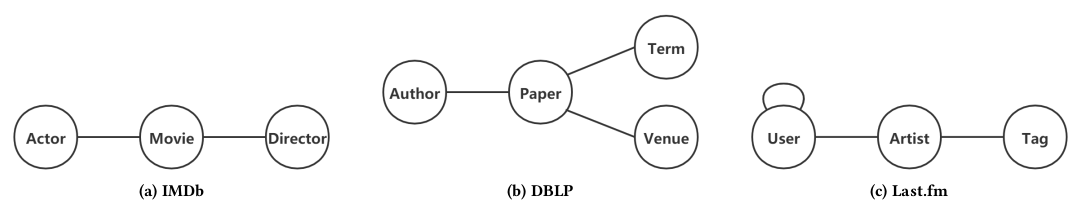
\includegraphics[width=\textwidth]{figs/fig3.png}
  \caption{Các lược đồ mạng của ba bộ dữ liệu đồ thị không đồng nhất được sử dụng trong bài viết này.}
\end{figure*}

\begin{itemize}
  \item $\mathbf{IMDb}^{1}$ là cơ sở dữ liệu trực tuyến về các bộ phim và chương trình truyền hình, bao gồm các thông tin như dàn diễn viên, đội ngũ sản xuất và tóm tắt cốt truyện. Chúng tôi sử dụng một tập mẫu được lấy ra từ IMDb, thông qua quá trình tiền xử lí dữ liệu thu được 4278 bộ phim, 2081 đạo diễn và 5257 diễn viên. Phim được gắn nhãn là một trong ba loại (Hành động, Hài kịch và Chính kịch) dựa trên thông tin thể loại của chúng. Mỗi bộ phim cũng được mô tả bằng một bag-of-words đại diện cho các từ khóa cốt truyện của chúng. Đối với các mô hình học bán giám sát, các nút phim được chia thành các tập huấn luyện, xác thực và kiểm tra với kích thước lần lượt là 400 (9,35\%), 400 (9,35\%) và $3478(81,30 \%)$ nút.
  \item $\mathbf{DBLPP}^{2}$ là một trang web tổng hợp danh mục tài liệu về khoa học máy tính. Chúng tôi sử dụng một tập mẫu được lấy ra từ DBLP [12, 15], sau khi tiền xử lí dữ liệu thu được thông tin về 4057 tác giả, 14328 bài báo, 7723 thuật ngữ và 20 nơi xuất bản. Các tác giả được chia thành bốn lĩnh vực nghiên cứu (Cơ sở dữ liệu, Khai thác dữ liệu, Trí tuệ nhân tạo và Truy xuất thông tin). Mỗi tác giả được mô tả bằng một bag-of-words đại diện cho các từ khóa trong bài báo của họ. Đối với các mô hình học bán giám sát, các nút tác giả được chia thành các tập huấn luyện, xác thực và kiểm tra với kích thước lần lượt là $400(9,86 \%)$ 400 (9,86\%) và 3257 (80,28\%) nút.
  \item $\mathbf{Last.fm}^{3}$ là trang web âm nhạc theo dõi thông tin hành vi nghe nhạc của người dùng từ nhiều nguồn khác nhau. Chúng tôi sử dụng bộ dữ liệu do HetRec 2011 phát hành [4], sau khi tiền xử lí dữ liệu thu được thông tin về 1892 người dùng, 17632 nghệ sĩ và 1088 thẻ nghệ sĩ. Tập dữ liệu này được sử dụng cho tác vụ dự đoán liên kết giữa các nút, trong đó tập dữ liệu không chứa bất cứ thông tin nào liên quan đến nhãn hay các đặc điểm đặc trưng của đối tượng. Đối với các mô hình học bán giám sát, các cặp người dùng - nghệ sĩ được chia thành các tập huấn luyện, xác thực và kiểm tra với kích thước lần lượt là $64984(70 \%), 9283(10 \%)$ và $18567(20 \%)$ cặp.
\end{itemize}

\subsection{Các mô hình tham chiếu}
Chúng tôi so sánh MAGNN với nhiều loại mô hình biểu diễn đồ thị khác nhau, bao gồm các mô hình biểu diễn đồ thị đồng nhất truyền thống (trái ngược với GNN), mô hình biểu diễn đồ thị không đồng nhất truyền thống, GNN cho đồ thị đồng nhất và GNN cho đồ thị không đồng nhất. Ta gọi chúng lần lượt là mô hình đồng nhất truyền thống, mô hình không đồng nhất truyền thống, GNN đồng nhất và GNN không đồng nhất. Danh sách các mô hình tham chiếu cơ sở được thể hiện dưới đây.

\begin{table}[]
  \label{tb:02}
  \caption{Thống kê mô tả các tập dữ liệu}
  \begin{tabular}{|l|l|l|l|}
  \hline
  Dữ liệu & Nút                                                                                                                                     & Cạnh                                                                                     & Metapath                                                                      \\ \hline
  IMDb    & \begin{tabular}[c]{@{}l@{}}\# phim (M): 4278\\ \# đạo diễn (D): 2081\\ \# diễn viên (A): 5257\end{tabular}                              & \begin{tabular}[c]{@{}l@{}}\# M-D: 4278\\ \# M-A: 12828\end{tabular}                     & \begin{tabular}[c]{@{}l@{}}MDM\\ MAM\\ DMD\\ DMAMD\\ AMA\\ AMDMA\end{tabular} \\ \hline
  DBLP    & \begin{tabular}[c]{@{}l@{}}\# tác giả (A): 4057\\ \# bài báo (P): 14328\\ \# thuật ngữ (T): 7723\\ \# nới xuất bản (V): 20\end{tabular} & \begin{tabular}[c]{@{}l@{}}\# A-P: 19645\\ \# P-T: 85810\\ \# P-V: 14328\end{tabular}    & \begin{tabular}[c]{@{}l@{}}APA\\ APTPA\\ APVPA\end{tabular}                   \\ \hline
  Last.fm & \begin{tabular}[c]{@{}l@{}}\# người dùng (U): 1892\\ \# nghệ sĩ (A): 17632\\ \# thẻ (T): 1088\end{tabular}                              & \begin{tabular}[c]{@{}l@{}}\# U-U: 12,717\\ \# U-A: 92,834\\ \# A-T: 23,253\end{tabular} & \begin{tabular}[c]{@{}l@{}}UU\\ UAU\\ UATAU\\ AUA\\ AUUA\\ ATA\end{tabular}   \\ \hline
  \end{tabular}
  \end{table}

\begin{itemize}
  \item $\mathbf{LINE}$ [25] là một mô hình đồng nhất truyền thống khai thác mức độ tương đồng bậc nhất và bậc hai giữa các nút. Chúng tôi áp dụng mô hình này cho các đồ thị không đồng nhất bằng cách bỏ qua tính không đồng nhất của cấu trúc đồ thị và loại bỏ tất cả các thuộc tính liên quan đến nội dung nút. Trong các thử nghiệm của tác giả, chúng tôi sử dụng biến thể LINE (sử dụng mức độ tương đồng bậc hai).
  \item $\mathbf{node2vec}$ [13] là một mô hình đồng nhất truyền thống và có thể coi là phiên bản tổng quát của DeepWalk [21]. Chúng tôi áp dụng mô hình này cho các đồ thị không đồng nhất theo cách tương tự như LINE.
  \item $\mathbf{ESim}$ [22] là một mô hình không đồng nhất truyền thống học cách biểu diễn nút từ các cấu hình metapath đã được lấy mẫu. ESim yêu cầu xác định trước các trọng số cho mỗi metapath. Ở đây, chúng tôi chỉ định các trọng số bằng nhau cho tất cả các metapath vì việc tìm kiếm các trọng số tối ưu của các metapath là rất khó và không mang lại mức tăng hiệu suất đáng kể so với việc đặt các trọng số mặc định bằng nhau theo các thử nghiệm của nhóm tác giả.
  \item $\mathbf{metapath2vec}$ [9] là một mô hình không đồng nhất truyền thống tạo ra các biểu diễn nút bằng cách cung cấp các random walks được định hướng bởi metapath cho một mô hình skip-gram. Mô hình này dựa trên một metapath do người dùng chỉ định, vì vậy chúng tôi thử nghiệm trên tất cả các metapath riêng biệt và tổng kết metapath có kết quả tốt nhất. Chúng tôi sử dụng biến thể metapath2vec++ trong các thử nghiệm của mình. 
  \item $\mathbf{HERec}$ [23] là một mô hình không đồng nhất truyền thống học cách biểu diễn nút bằng cách áp dụng DeepWalk cho các đồ thị đồng nhất dựa trên metapath được chuyển đổi từ đồ thị không đồng nhất ban đầu. Mô hình này đi kèm với một thuật toán kết hợp biểu diễn được thiết kế để dự đoán xếp hạng, có thể được điều chỉnh để dự đoán liên kết. Để phân loại/phân cụm nút, chúng tôi chọn và báo cáo kết quả cho metapath có hiệu suất tốt nhất.
  \item $\mathbf{GCN}$ [16] là một mô hình GNN đồng nhất. Mô hình này thực hiện các phép toán tích chập trong miền Fourier của đồ thị. Ở đây, chúng tôi kiểm tra hiệu suất của GCN trên các đồ thị đồng nhất dựa trên metapath và báo cáo kết quả cho metapath tốt nhất.
  \item $\mathbf{GAT}$ [28] là một GNN đồng nhất. Mô hình này thực hiện các thao tác tích chập trong miền không gian đồ thị với cơ chế kết hợp có chú ý. Tương tự, ở đây chúng tôi kiểm tra GAT trên các đồ thị đồng nhất dựa trên metapath và báo cáo kết quả cho metapath tốt nhất.
  \item $\mathbf{GATNE}$ [5] là một GNN không đồng nhất. Mô hình này tạo ra biểu diễn của nút từ biểu diễn cơ sở và biểu diễn cạnh, tập trung vào nhiệm vụ dự đoán liên kết. Ở đây chúng tôi báo cáo kết quả từ biến thể GATNE có hiệu quả tốt nhất.
  \item $\mathbf{HAN}$ [31] là một GNN không đồng nhất. Mô hình này học cách biểu diễn nút với metapath cụ thể từ các đồ thị đồng nhất khác nhau dựa trên metapath và tận dụng cơ chế chú ý để kết hợp chúng thành một biểu diễn vectơ cho mỗi nút.
\end{itemize}

% \usepackage{tabularray}
\begin{table*}[t]
  \label{tb:03}
  \caption{Kết quả thực nghiệm}
  \centering
  \begin{tblr}{
    cells = {c},
    cell{1}{1} = {r=2}{},
    cell{1}{2} = {r=2}{},
    cell{1}{3} = {r=2}{},
    cell{1}{4} = {c=5}{},
    cell{1}{9} = {c=4}{},
    cell{3}{1} = {r=8}{},
    cell{3}{2} = {r=4}{},
    cell{7}{2} = {r=4}{},
    cell{11}{1} = {r=8}{},
    cell{11}{2} = {r=4}{},
    cell{15}{2} = {r=4}{},
    vlines,
    hline{1,3,11,19} = {-}{},
    hline{2} = {4-12}{},
    hline{4-6,8-10,12-14,16-18} = {3-12}{},
    hline{7,15} = {2-12}{},
  }
  Tập dữ liệu & Độ đo    & Train \% & Không giám sát &          &       &              &       & Bán giám sát &       &       &       \\
              &          &          & LINE           & node2vec & ESim  & metapath2vec & HERec & GCN          & GAT   & HAN   & MAGNN \\
  IMDb        & Macro-F1 & $20 \%$  & 44.04          & 49.00    & 48.37 & 46.05        & 45.61 & 52.73        & 53.64 & 56.19 & 59.35 \\
              &          & $40 \%$  & 45.45          & 50.63    & 50.09 & 47.57        & 46.80 & 53.67        & 55.50 & 56.15 & 60.27 \\
              &          & $60 \%$  & 47.09          & 51.65    & 51.45 & 48.17        & 46.84 & 54.24        & 56.46 & 57.29 & 60.66 \\
              &          & $80 \%$  & 47.49          & 51.49    & 51.37 & 49.99        & 47.73 & 54.77        & 57.43 & 58.51 & 61.44 \\
              & Micro-F1 & $20 \%$  & 45.21          & 49.94    & 49.32 & 47.22        & 46.23 & 52.80        & 53.64 & 56.32 & 59.60 \\
              &          & $40 \%$  & 46.92          & 51.77    & 51.21 & 48.17        & 47.89 & 53.76        & 55.56 & 57.32 & 60.50 \\
              &          & $60 \%$  & 48.35          & 52.79    & 52.53 & 49.87        & 48.19 & 54.23        & 56.47 & 58.42 & 60.88 \\
              &          & $80 \%$  & 48.98          & 52.72    & 52.54 & 50.50        & 49.11 & 54.63        & 57.40 & 59.24 & 61.53 \\
  DBLP        & Macro-F1 & $20 \%$  & 87.16          & 86.70    & 90.68 & 88.47        & 90.82 & 88.00        & 91.05 & 91.69 & 93.13 \\
              &          & $40 \%$  & 88.85          & 88.07    & 91.61 & 89.91        & 91.44 & 89.00        & 91.24 & 91.96 & 93.23 \\
              &          & $60 \%$  & 88.93          & 88.69    & 91.84 & 90.50        & 92.08 & 89.43        & 91.42 & 92.14 & 93.57 \\
              &          & $80 \%$  & 89.51          & 88.93    & 92.27 & 90.86        & 92.25 & 89.98        & 91.73 & 92.50 & 94.10 \\
              & Micro-F1 & $20 \%$  & 87.68          & 87.21    & 91.21 & 89.02        & 91.49 & 88.51        & 91.61 & 92.33 & 93.61 \\
              &          & $40 \%$  & 89.25          & 88.51    & 92.05 & 90.36        & 92.05 & 89.22        & 91.77 & 92.57 & 93.68 \\
              &          & $60 \%$  & 89.34          & 89.09    & 92.28 & 90.94        & 92.66 & 89.57        & 91.97 & 92.72 & 93.99 \\
              &          & $80 \%$  & 89.96          & 89.37    & 92.68 & 91.31        & 92.78 & 90.33        & 92.24 & 93.23 & 94.47 
  \end{tblr}
\end{table*}

Đối với các mô hình truyền thống, bao gồm LINE, node2vec, ESim, metapath2vec và HERec, chúng tôi thiết lập window size là 5, walk length là 100, số bước đi trên mỗi nút là 40 và số lượng mẫu âm tính là 5 (nếu có). Đối với các mô hình GNN (bao gồm GCN, GAT, HAN và MAGNN), chúng tôi đặt tỷ lệ dropout là 0,5; chúng tôi sử dụng tập dữ liệu huấn luyện, xác thực và kiểm tra có kích thước bằng nhau; chúng tôi sử dụng phương pháp Adam cho các nhiệm vụ tối ưu hóa với learning rate được thiết lập là 0,005 và tham số phân rã (L2) được đặt là 0,001; chúng tôi huấn luyện mô hình GNN trong 100 epochs và cho phép dừng sớm với ngưỡng patience là 30. Để phân loại nút và phân cụm nút, GNN được huấn luyện theo kiểu bán giám sát với một phần nhỏ các nút được gắn nhãn. Đối với GAT, HAN và MAGNN, chúng tôi thiết lập số lượng head chú ý là 8. Đối với HAN và MAGNN, chúng tôi thiết lập số chiều (thứ nguyên) của vectơ chú ý trong tập hợp giữa các metapath là 128. Để việc so sánh được công bằng, chúng tôi đặt số chiều (thứ nguyên) biểu diễn của tất cả các mô hình được đề cập ở trên đến 64.

\subsection{Phân loại nút (RQ1)}
Chúng tôi tiến hành thử nghiệm trên tập dữ liệu IMDb và DBLP để so sánh hiệu quả của các mô hình khác nhau đối với tác vụ phân loại nút. Chúng tôi sử dụng thông tin biểu diễn của các nút được gắn nhãn (phim trong IMDb và tác giả trong DBLP) được tạo ra bởi mỗi mô hình làm đầu vào cho thuật toán phân loại SVM với các tỷ lệ tập huấn luyện khác nhau. Để việc so sánh được công bằng, chỉ các nút trong tập kiểm tra (testing set) được đưa vào mô hình SVM, bởi vì các mô hình bán giám sát đã được học thông tin từ các nút trong tập huấn luyện (training set) và xác thực (validation sey), như được thể hiển trong Phương trình (11). Do đó, tỉ lệ tập huấn luyện và kiểm tra của mô hình SVM ở đây chỉ liên quan đến tập dữ liệu kiểm tra (nghĩa là 3478 nút cho IMDb và 3257 nút cho DBLP). Việc phân chia tập train và test cho mô hình SVM cũng được thực hiện tương tự nhau giữa các mô hình biểu diễn đồ thị. Các chiến lược tương tự cũng được áp dụng cho các thử nghiệm liên quan đến bài toán phân cụm nút và dự đoán liên kết. Chúng tôi tổng kết giá trị Macro-F1 và Micro-F1 trung bình của 10 lần chạy của từng mô hình biểu diễn trong Bảng 3.

Như được thể hiện trong bảng, MAGNN luôn hiệu quả hơn so với các mô hình tham chiếu khác trên các tỷ lệ tập dữ liệu huấn luyện khác nhau. Trên tập dữ liệu IMDb, thật thú vị khi thấy rằng node2vec hoạt động tốt hơn các mô hình không đồng nhất truyền thống. Điều đó cho thấy rằng, các mô hình GNN nói chung và đặc biệt là các mô hình GNN không đồng nhất nói riêng có thể giúp thu được các kết quả tốt hơn, chứng tỏ rằng kiến trúc GNN, sử dụng một cách thận trọng các đặc trưng của nút không đồng nhất, giúp cải thiện hiệu quả của việc biểu diễn đồ thị. Mức tăng hiệu suất mà MAGNN mang lại so với mô hình tham chiếu tốt nhất (HAN) là khoảng 4-7\%, điều này cho thấy rằng các cấu hình metapath chứa đựng nhiều thông tin phong phú hơn so với các lân cận dựa metapath. Trên tập dữ liệu DBLP, việc phân loại nút là một nhiệm vụ không quá quan trọng, điều này có thể thấy được thông qua việc tất cả các mô hình đều có thể đạt được các chỉ số tốt cho bài toán này. Mặc dù vậy, MAGNN vẫn vượt trội so với các mô hình tham chiếu tốt nhất $1-2 \%$.

\begin{table*}[t]
  \label{tb:04}
  \caption{Kết quả thực nghiệm (\%) trên tập dữ liệu IMDb và DBLP đối với tác vụ phân cụm nút}
  \centering
  \begin{tblr}{
    cells = {c},
    cell{1}{1} = {r=2}{},
    cell{1}{2} = {r=2}{},
    cell{1}{3} = {c=4}{},
    cell{1}{7} = {c=4}{},
    cell{3}{1} = {r=2}{},
    cell{5}{1} = {r=2}{},
    vlines,
    hline{1,3,5,7} = {-}{},
    hline{2} = {3-11}{},
    hline{4,6} = {2-11}{},
  }
  Tập dữ liệu & Độ đo & Không giám sát &          &       &              & Bán giám sát &       &       &       &                      \\
              &       & LINE           & node2vec & ESim  & metapath2vec & HERec        & GCN   & GAT   & HAN   & MAGNN                \\
  IMDb        & NMI   & 1.13           & 5.22     & 1.07  & 0.89         & 0.39         & 7.46  & 7.84  & 10.79 & $\mathbf{1 5 . 5 8}$ \\
              & ARI   & 1.20           & 6.02     & 1.01  & 0.22         & 0.11         & 7.69  & 8.87  & 11.11 & $\mathbf{1 6 . 7 4}$ \\
  DBLP        & NMI   & 71.02          & 77.01    & 68.33 & 74.18        & 69.03        & 73.45 & 70.73 & 77.49 & $\mathbf{8 0 . 8 1}$ \\
              & ARI   & 76.52          & 81.37    & 72.22 & 78.11        & 72.45        & 77.50 & 76.04 & 82.95 & $\mathbf{8 5 . 5 4}$ 
  \end{tblr}
  \end{table*}

\begin{table*}[t]
  \label{tb:05}
  \caption{Kết quả thực nghiệm (\%) trên tập dữ liệu Last.fm đối với tác vụ dữ đoán liên kết}
  \centering
  \begin{tblr}{
    cells = {c},
    cell{2}{1} = {r=2}{},
    vlines,
    hline{1-2,4} = {-}{},
    hline{3} = {2-11}{},
  }
  Dataset & Metrics & LINE  & node2vec & ESim  & metapath2vec & HERec & GCN   & GAT   & GATNE & HAN   & MAGNN                \\
  Last.fm & AUC     & 85.76 & 67.14    & 82.00 & 92.20        & 91.52 & 90.97 & 92.36 & 89.21 & 93.40 & $\mathbf{9 8 . 9 1}$ \\
          & AP      & 88.07 & 64.11    & 82.19 & 90.11        & 89.47 & 91.65 & 91.55 & 88.86 & 92.44 & $\mathbf{9 8 . 9 3}$ 
  \end{tblr}
\end{table*}


\subsection{Phân cụm nút (RQ2)}
Chúng tôi tiến hành thử nghiệm trên tập dữ liệu IMDb và DBLP để so sánh hiệu quả của các mô hình khác nhau trong tác vụ phân cụm nút. Chúng tôi sử dụng thông tin biểu diễn của các nút được gắn nhãn (phim trong IMDb và tác giả trong DBLP) được tạo bởi từng mô hình học máy làm thông tin đầu vào cho thuật toán phân cụm K-Means. Số cụm trong K-Means được chọn là số lớp cho mỗi tập dữ liệu, tức là 3 cụm cho tập dữ liệu IMDb và 4 cụm cho tập dữ liệu DBLP. Chúng tôi sử dụng NMI (normalized mutual information - thông tin chung đã chuẩn hóa) và chỉ số ARI làm độ đo chính. Do kết quả phân cụm của thuật toán K-Means phụ thuộc rất nhiều vào quá trình khởi tạo tâm cụm nên chúng tôi lặp lại thuật toán K-Means 10 lần cho mỗi lần chạy mô hình biểu diễn đồ thị và mỗi mô hình biểu diễn đồ thị được đánh giá trong 10 lần chạy. C kết quả trung bình thu được từ các lần chạy được thể hiện trong Bảng 4.

Từ Bảng 4, chúng ta có thể thấy rằng MAGNN luôn vượt trội so với tất cả các mô hình tham chiếu khác trong việc phân cụm nút. Lưu ý rằng tất cả các mô hình có hiệu suất trên tập dữ liệu IMDb kém hơn nhiều so với trên tập dữ liệu DBLP. Điều này có thể do nhãn bẩn (dirty labels) của các bộ phim trong tập dữ liệu IMDb: mỗi nút bộ phim trong bộ dữ liệu IMDb gốc có nhiều thể loại và chúng tôi chỉ chọn loại đầu tiên làm nhãn lớp của chúng. Chúng ta có thể thấy rằng các mô hình không đồng nhất truyền thống không có nhiều ưu điểm so với các mô hình đồng nhất truyền thống trong việc phân cụm nút. Node2vec được cho là sẽ hiệu quả rõ rệt trong tác vụ phân cụm nút bởi vì đây là một cách tiếp cận dựa trên random walk, vì vậy nó buộc các nút ở gần nhau trên đồ thị cũng phải ở gần nhau trong không gian biểu diễn [33] và từ đó có thể mã hóa được thông tin vị trí của nút. Đặc điểm này vô cùng thuận lợi cho thuật toán K-Means vì nó phải phân cụm các nút dựa trên khoảng cách Euclide giữa các điểm biểu biễn. Mặc dù vậy, các GNN nhận biết tính không đồng nhất (tức là HAN và MAGNN) vẫn dẫn đầu về hiệu quả trong việc phân cụm nút trên cả hai bộ dữ liệu.

\subsection{Dự đoán liên kết (RQ3)}
Chúng tôi cũng tiến hành thử nghiệm trên tập dữ liệu Last.fm để đánh giá hiệu quả của MAGNN và các mô hình tham chiếu khác đối với tác vụ dự đoán liên kết. Đối với các mô hình GNN, chúng tôi coi cặp người dùng-nghệ sĩ được kết nối là các cặp nút positive và coi tất cả các liên kết người dùng-nghệ sĩ không được kết nối là các cặp nút negative. Chúng tôi thêm cùng một số cặp nút negative được lấy mẫu ngẫu nhiên vào tập validation và tập testing. Trong quá trình huấn luyện mô hình GNN, các cặp nút negative cũng được lấy mẫu theo phân phối đều. Các mô hình GNN sau đó được tối ưu hóa bằng cách tối thiểu hóa hàm mục tiêu đã mô tả trong Công thức (12). Với mỗi biểu diễn của nút người dùng $\mathbf{h}_{u}$ và nút nghệ sĩ $\mathbf{h}_{a}$ 
do mô hình tạo ra, ta tính xác suất để $u$ và $v$ liên kết với nhau như sau:

\begin{equation}
  p_{u a}=\sigma\left(\mathbf{h}_{u}^{\top} \cdot \mathbf{h}_{a}\right)
\end{equation}
trong đó $\sigma(\cdot)$ là hàm sigmoid. Các mô hình biểu diễn đồ thị để dự đoán liên kết được đánh giá theo AUC (diện tích phía dưới đường cong ROC) và độ chính xác trung bình (AP). Chúng tôi tổng kết kết quả trung bình của 10 lần chạy ứng với từng mô hình biểu diễn đồ thị trong Bảng 5. 

Từ Bảng 5, có thể thấy MAGNN vượt trội hơn rõ rệt so với các mô hình tham chiếu khác. Mô hình truyền thống mạnh nhất ở đây là metapath2vec, mô hình này học từ các chuỗi nút được tạo từ các random walk được định hướng bởi một metapath duy nhất. MAGNN đạt được các chỉ số cao hơn so với metapath2vec, cho thấy rằng việc xem xét một metapath duy nhất là không hoàn toàn tối ưu. Trong số các mô hình tham chiếu có dạng GNN, HAN thu được kết quả tốt nhất vì nó nhận biết được tính không đồng nhất và kết hợp nhiều metapath. MAGNN đạt được mức cải thiện xấp xỉ khoảng $6 \%$ so với HAN. Kết quả này một lần nữa giúp củng cố thêm cho khẳng định của nhóm tác giả rằng  metapath context của các nút là rất quan trọng đối với việc biểu diễn nút.

% \usepackage{tabularray}
\begin{table*}[t]
  \label{tb:06}
  \caption{Kết quả phân tích ảnh hưởng của từng thành phần}
  \centering
  \begin{tblr}{
    row{2} = {c},
    cell{1}{1} = {r=2}{},
    cell{1}{2} = {c=4}{c},
    cell{1}{6} = {c=4}{c},
    cell{1}{10} = {c=2}{c},
    cell{3}{2} = {c},
    cell{3}{3} = {c},
    cell{3}{4} = {c},
    cell{3}{5} = {c},
    cell{3}{6} = {c},
    cell{3}{7} = {c},
    cell{3}{8} = {c},
    cell{3}{9} = {c},
    cell{3}{10} = {c},
    cell{3}{11} = {c},
    cell{4}{2} = {c},
    cell{4}{3} = {c},
    cell{4}{4} = {c},
    cell{4}{5} = {c},
    cell{4}{6} = {c},
    cell{4}{7} = {c},
    cell{4}{8} = {c},
    cell{4}{9} = {c},
    cell{4}{10} = {c},
    cell{4}{11} = {c},
    cell{5}{2} = {c},
    cell{5}{3} = {c},
    cell{5}{4} = {c},
    cell{5}{5} = {c},
    cell{5}{6} = {c},
    cell{5}{7} = {c},
    cell{5}{8} = {c},
    cell{5}{9} = {c},
    cell{5}{10} = {c},
    cell{5}{11} = {c},
    cell{6}{2} = {c},
    cell{6}{3} = {c},
    cell{6}{4} = {c},
    cell{6}{5} = {c},
    cell{6}{6} = {c},
    cell{6}{7} = {c},
    cell{6}{8} = {c},
    cell{6}{9} = {c},
    cell{6}{10} = {c},
    cell{6}{11} = {c},
    cell{7}{2} = {c},
    cell{7}{3} = {c},
    cell{7}{4} = {c},
    cell{7}{5} = {c},
    cell{7}{6} = {c},
    cell{7}{7} = {c},
    cell{7}{8} = {c},
    cell{7}{9} = {c},
    cell{7}{10} = {c},
    cell{7}{11} = {c},
    cell{8}{2} = {c},
    cell{8}{3} = {c},
    cell{8}{4} = {c},
    cell{8}{5} = {c},
    cell{8}{6} = {c},
    cell{8}{7} = {c},
    cell{8}{8} = {c},
    cell{8}{9} = {c},
    cell{8}{10} = {c},
    cell{8}{11} = {c},
    vlines,
    hline{1,3-9} = {-}{},
    hline{2} = {2-11}{},
  }
  Variant                  & IMDb                 &                      &                      &                      & DBLP                 &                      &                      &                      & Last.fm              &                      \\
                           & Macro-F1             & Micro-F1             & NMI                  & ARI                  & Macro-F1             & Micro-F1             & NMI                  & ARI                  & AUC                  & AP                   \\
  MAGNN $_\text {feat }$   & 48.87                & 50.36                & 5.82                 & 5.30                 & 92.80                & 93.32                & 77.17                & 82.15                & N/A                  & N/A                  \\
  MAGNN $_\text {nb }$     & 58.45                & 58.84                & 12.87                & 11.98                & 92.61                & 93.15                & 77.64                & 82.60                & 93.68                & 92.95                \\
  MAGNN $_\text {sm }$     & 56.77                & 56.64                & 11.90                & 11.84                & 93.19                & 93.69                & 79.48                & 84.39                & 92.54                & 91.52                \\
  MAGNN $_\text {avg }$    & 59.66                & 59.78                & 13.64                & 15.27                & 93.13                & 93.44                & 79.31                & 84.30                & 98.63                & 98.57                \\
  MAGNN $_\text {linear }$ & 57.80                & 57.96                & 9.80                 & 8.49                 & 93.21                & 93.52                & 78.95                & 83.89                & 98.56                & 98.48                \\
  MAGNN $_\text {rot }$    & $\mathbf{6 0 . 4 3}$ & $\mathbf{6 0 . 6 3}$ & $\mathbf{1 5 . 5 8}$ & $\mathbf{1 6 . 7 4}$ & $\mathbf{9 3 . 5 1}$ & $\mathbf{9 3 . 9 4}$ & $\mathbf{8 0 . 8 1}$ & $\mathbf{8 5 . 5 4}$ & $\mathbf{9 8 . 9 1}$ & $\mathbf{9 8 . 9 3}$ 
  \end{tblr}
\end{table*}

\subsection{Nghiên cứu phân tách ảnh hưởng của từng thành phần trong MAGNN (RQ4)}
Để xác thực tính hiệu quả của từng thành phần trong mô hình của chúng tôi, chúng tôi tiếp tục tiến hành thử nghiệm trên các biến thể MAGNN khác nhau. Trong phạm vi báo cáo này, chúng tôi tổng hợp kết quả thu được từ ba bộ dữ liệu trên cả ba nhiệm vụ trong Bảng 6. Lưu ý rằng tất cả các chỉ số được thể hiện đối với tác vụ phân loại nút (tức là Macro-F1 và Micro-F1) là giá trị trung bình của các chỉ số theo các tỷ lệ tập huấn luyện khác nhau (giải thích chi tiết trong Mục V.C). Ở đây $\mathbf{MAGNN}_{rot}$ là mô hình được đề xuất của chúng tôi sử dụng bộ mã hóa dựa trên phép quay quan hệ, tức là mô hình được sử dụng để cạnh tranh với các mô hình tham chiếu khác trong Bảng 3, 4 và 5. Gọi $\mathbf{MAGNN}_{rot}$ là mô hình tham chiếu, $\mathbf{MAGNN}_{feat}$ là mô hình tương đương mà không sử dụng các đặc trưng về nội dung của nút; $\mathbf{MAGNN}_{nb}$ chỉ xem xét các nút lân cận dựa trên metapath; $\mathbf{MAGNN}_{sm}$ chỉ xem xét một metapath tốt nhất; $\mathbf{MAGNN}_{avg}$ chuyển sang sử dụng mã hóa tuyến tính cấu hình metapath. Ngoại trừ những khác biệt nêu trên, tất cả các cài đặt khác đều giống nhau đối với các biến thể MAGNN này. Lưu ý rằng $\mathbf{MAGNN}_{feat}$ trên tập dữ liệu Last.fm tương đương với $\mathbf{MAGNN}_{rot}$ vì tập dữ liệu này không chứa các thuộc tính của nút.

Có thể thấy, bằng cách sử dụng các thuộc tính nội dung nút, $\mathbf{MAGNN}_{rot}$ đạt được sự cải thiện hiệu suất đáng kể so với $\mathbf{MAGNN}_{feat}$, điều này cho thấy sự cần thiết của việc biến đổi nội dung nút để kết hợp với các đặc trưng khác của nút. So sánh $\mathbf{MAGNN}_{nb}$ với $\mathbf{MAGNN}_{avg}$, $\mathbf{MAGNN}_{linear}$ và $\mathbf{MAGNN}_{rot}$, ta thấy rằng việc tổng hợp các cấu hình metapath thay vì tìm các lân cận dựa trên metapath mang lại sự gia tăng về hiệu suất, điều này xác nhận tính hiệu quả của việc tổng hợp intra-metapath. Bên cạnh đó, sự khác biệt giữa kết quả của $\mathbf{MAGNN}_{sm}$ và $\mathbf{MAGNN}_{rot}$ cho thấy rằng hiệu suất của mô hình được cải thiện đáng kể bằng cách kết hợp nhiều metapath trong quá trình tổng hợp inter-metapath. Cuối cùng, kết quả của $\mathbf{MAGNN}_{avg}$, $\mathbf{MAGNN}_{linear}$ và $\mathbf{MAGNN}_{rot}$ cho thấy rằng cách mã hóa dựa trên phép quay quan hệ giúp cải thiện MAGNN một lượng nhỏ. Đáng chú ý là $\mathbf{MAGNN}_{linear}$ lại kém hiệu quả hơn $\mathbf{MAGNN}_{avg}$. Tuy nhiên, cả ba biến thể MAGNN sử dụng các bộ mã hóa khác nhau vẫn luôn hoạt động tốt hơn so với mô hình tham chiếu tốt nhất, HAN.

\subsection{Trực quan hóa (RQ5)}
Ngoài các đánh giá định lượng trên về các mô hình biểu diễn đồ thị, chúng tôi cũng trực quan hóa các cách biểu diễn nút để tiến hành đánh giá định tính các kết quả biểu diễn đồ thị. Chúng tôi chọn ngẫu nhiên 30 cặp người dùng-nghệ sĩ từ tập test có nhãn positive trong bộ dữ liệu Last.fm, sau đó chiếu kết quả biểu diễn của các nút này vào không gian 2 chiều bằng cách sử dụng phương pháp t-SNE. Trong phần này, chúng tôi minh họa kết quả trực quan hóa của LINE, ESim, GCN và MAGNN trong Hình 4, trong đó các điểm màu đỏ và điểm màu xanh lá cây lần lượt biểu thị người dùng và nghệ sĩ.

Dựa trên hình ảnh trực quan này, ta có thể nhanh chóng nhận ra sự khác biệt giữa các mô hình biểu diễn đồ thị về khả năng học của chúng đối với các đồ thị không đồng nhất. Là một mô hình biểu diễn đồ thị đồng nhất truyền thống, LINE không thể phân chia nút người dùng và nút nghệ sĩ thành hai nhóm khác nhau một cách hiệu quả. Ngược lại, ESim, một mô hình không đồng nhất truyền thống, có thể phân vùng gần đúng hai loại nút. Nhờ kiến trúc GNN mạnh mẽ và bằng cách chọn các metapath phù hợp, một mô hình GNN đồng nhất như GCN có thể cô lập các loại nút khác nhau và mã hóa thông tin tương quan của các cặp nghệ sĩ-người dùng vào các biểu diễn nút. Từ Hình 4, chúng ta có thể thấy rằng mô hình MAGNN mà chúng tôi đề xuất thu được kết quả biểu diễn đồ thị tốt nhất, với hai nhóm người dùng và nghệ sĩ được phân tách rõ ràng và mối tương quan phù hợp của các cặp nghệ sĩ-người dùng.


\section{Kết luận}



\begin{thebibliography}{00}
\bibitem{b1} G. Eason, B. Noble, and I. N. Sneddon, ``On certain integrals of Lipschitz-Hankel type involving products of Bessel functions,'' Phil. Trans. Roy. Soc. London, vol. A247, pp. 529--551, April 1955.
\bibitem{b2} J. Clerk Maxwell, A Treatise on Electricity and Magnetism, 3rd ed., vol. 2. Oxford: Clarendon, 1892, pp.68--73.
\bibitem{b3} I. S. Jacobs and C. P. Bean, ``Fine particles, thin films and exchange anisotropy,'' in Magnetism, vol. III, G. T. Rado and H. Suhl, Eds. New York: Academic, 1963, pp. 271--350.
\bibitem{b4} K. Elissa, ``Title of paper if known,'' unpublished.
\bibitem{b5} R. Nicole, ``Title of paper with only first word capitalized,'' J. Name Stand. Abbrev., in press.
\bibitem{b6} Y. Yorozu, M. Hirano, K. Oka, and Y. Tagawa, ``Electron spectroscopy studies on magneto-optical media and plastic substrate interface,'' IEEE Transl. J. Magn. Japan, vol. 2, pp. 740--741, August 1987 [Digests 9th Annual Conf. Magnetics Japan, p. 301, 1982].
\bibitem{b7} M. Young, The Technical Writer's Handbook. Mill Valley, CA: University Science, 1989.
\end{thebibliography}
\vspace{12pt}
\color{red}
IEEE conference templates contain guidance text for composing and formatting conference papers. Please ensure that all template text is removed from your conference paper prior to submission to the conference. Failure to remove the template text from your paper may result in your paper not being published.

\end{document}
